\documentclass[aspectratio=169,11pt]{beamer}
\usepackage{amsmath,amssymb,booktabs,array}
\usepackage{tikz,pgfplots}
\pgfplotsset{compat=1.18}
\usetikzlibrary{arrows.meta,positioning,fit,backgrounds}
\definecolor{ink}{HTML}{525B63}
\definecolor{accent}{HTML}{007F8B}
\definecolor{secondary}{HTML}{A65432}
\definecolor{muted}{HTML}{77818A}
\usetheme{default}
\setbeamertemplate{navigation symbols}{}
\setbeamercolor{normal text}{fg=ink,bg=white}
\setbeamercolor{structure}{fg=accent}
\setbeamercolor{frametitle}{fg=ink}
\setbeamerfont{frametitle}{size=\Large,series=\mdseries}
\setbeamersize{text margin left=7mm,text margin right=7mm}
\setbeamertemplate{itemize item}{\color{accent}\small$\bullet$}
\setbeamertemplate{itemize subitem}{\color{accent}\scriptsize$\bullet$}
\setbeamertemplate{frametitle}{\vspace{4mm}\insertframetitle\par\vspace{3mm}}
\setbeamertemplate{footline}{%
  \hspace{7mm}{\color{muted}\tiny Price incorporation after scheduled releases}%
  \hfill{\color{muted}\tiny\insertframenumber}\hspace{5mm}\vspace{3mm}}
\addtobeamertemplate{itemize/enumerate body begin}{\setlength\itemsep{0.45em}}{}
\newcolumntype{L}[1]{>{\raggedright\arraybackslash}p{#1}}
\newcommand{\source}[1]{\par\vfill{\scriptsize\color{muted}#1}\par}
\newcommand{\heading}[1]{{\bfseries #1}\par\vspace{0.4em}}
\pgfplotsset{every axis/.append style={
  axis lines=left,grid=major,grid style={ink!12},
  tick label style={font=\scriptsize},label style={font=\small},
  legend style={font=\scriptsize,draw=none,fill=none},
  every axis plot/.append style={line width=1.3pt}}}
\hypersetup{pdftitle={Price incorporation after scheduled releases},
  pdfauthor={Ivaylo Staykov},pdfsubject={Research design and model specification}}
\title{Price incorporation after scheduled releases}
\author{Ivaylo Staykov}
\pdfstringdefDisableCommands{\def\translate#1{#1}}
\begin{document}

{\setbeamertemplate{footline}{}
\begin{frame}[plain]
\vspace{1.1cm}
{\color{accent}\rule{1.4cm}{2pt}}\par\vspace{0.6cm}
{\huge Price incorporation after\\[0.2em]scheduled macro releases}\par
\vspace{0.8cm}{\large A measurement study of BTCUSDT}\par\vspace{0.4cm}
Estimand, model and validation\par\vspace{0.8cm}
{\small Research design. No primary fit has run.}
\end{frame}}

\begin{frame}{Outline}
\heading{Part 1: Measurement and model}
\begin{enumerate}
\item Releases, prices and event time
\item Fraction of the move, response curve and half-time
\item Joint likelihood and partial pooling
\item Posterior inference and uncertainty
\end{enumerate}
\vspace{0.6cm}\heading{Part 2: Validation and interpretation}
\begin{enumerate}\setcounter{enumi}{4}
\item Pre-data checks and fit diagnostics
\item Robustness checks, outcome rules and limits
\end{enumerate}
\end{frame}

\begin{frame}{Motivation: separate speed from magnitude}
\begin{columns}[T,onlytextwidth]
\begin{column}{0.47\textwidth}\heading{Question}
\begin{itemize}
\item How much of a release-window price move occurs in the first seconds?
\item A large early move could mean a large response, a fast response, or both.
\item CPI and employment news can move prices in either direction.
\end{itemize}
\end{column}
\begin{column}{0.47\textwidth}\heading{Design}
\begin{itemize}
\item Anchor returns to a scheduled release time.
\item Estimate the signed magnitude and the rate separately for each event.
\item Pool event rates to estimate a population half-time.
\item Test whether its 95\% interval lies below 60 seconds.
\end{itemize}
\end{column}\end{columns}
\source{The question concerns repricing, not return prediction or a trading rule.}
\end{frame}

\begin{frame}{Data: scheduled releases in a continuously traded market}
\begin{columns}[T,onlytextwidth]
\begin{column}{0.48\textwidth}\heading{Primary sample}
\begin{itemize}
\item 106 CPI and 106 Employment Situation releases, scheduled at 08:30 ET.
\item 1 September 2017 to 31 July 2026; boundaries set by archive availability.
\item Dates from verified release calendars, not inferred from price jumps.
\end{itemize}
\end{column}
\begin{column}{0.46\textwidth}\heading{Prices and comparison sample}
\begin{itemize}
\item Binance BTCUSDT spot, one-second bars, publicly downloadable with checksums.
\item No market opening boundary at release time.
\item 71 FOMC statements fitted separately: the press conference contaminates the hour.
\end{itemize}
\end{column}\end{columns}
\source{212 is the calendar count before exclusions. The 2026-08-30 deviation corrects the preregistered 214.\\
Sources: ADRs 0001 to 0003; \texttt{release\_calendar.csv}. Other-agency release screening remains open (\#41).}
\end{frame}

\begin{frame}{Exploratory check: prices react at the release time}
\begin{columns}[c,onlytextwidth]
\begin{column}{0.63\textwidth}
\centering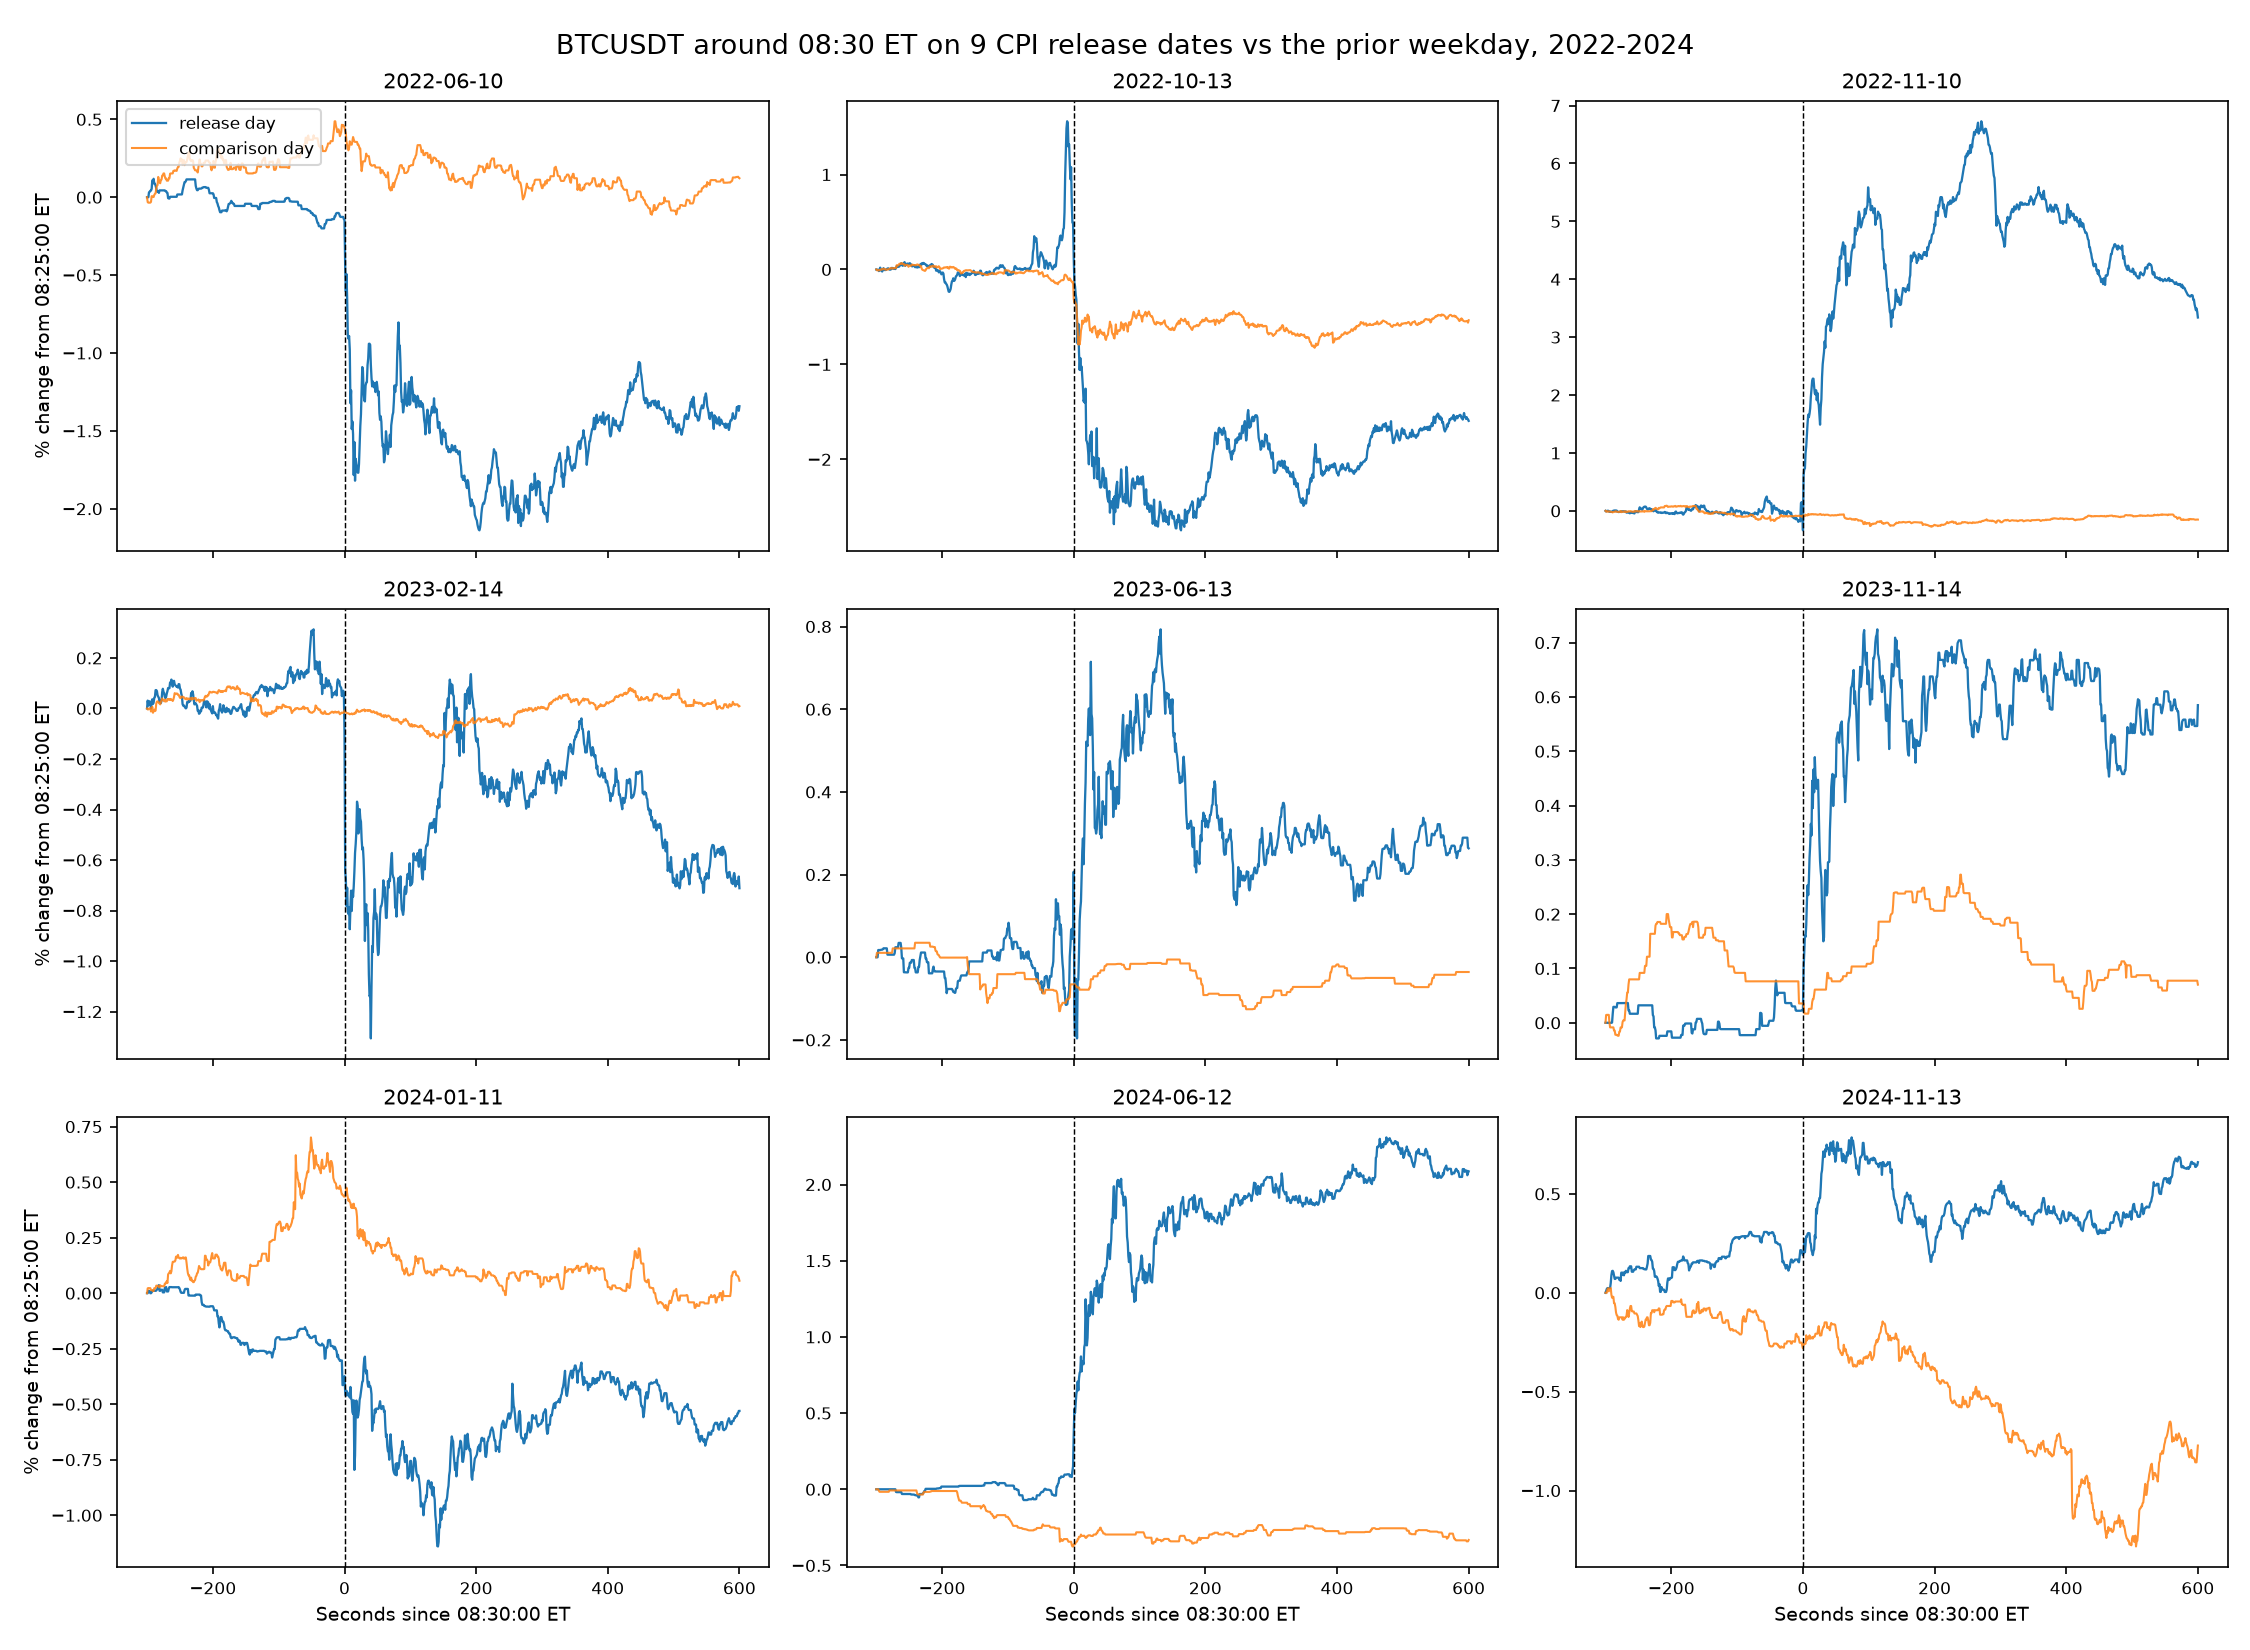
\includegraphics[width=\textwidth,height=0.64\textheight,keepaspectratio]{../../figures/spikeGrid.png}
\end{column}
\begin{column}{0.33\textwidth}\begin{itemize}
\item Nine CPI dates, each compared with the prior weekday at the same clock time.
\item This is not a half-time estimate or a representative sample.
\item These dates also informed the rate prior; that reuse is disclosed.
\end{itemize}\end{column}\end{columns}
\source{Source: \#6 and \texttt{notebooks/cpi-kill-check.ipynb}. The plot ends at 10 minutes, not one hour.}
\end{frame}

\begin{frame}{Event time: one second means one elapsed second}
\begin{columns}[T,onlytextwidth]
\begin{column}{0.47\textwidth}\begin{itemize}
\item Release $e$ occurs at $t_e$; event time is $\tau=t-t_e$, in seconds.
\item $P_e(0^-)$ is the last traded price strictly before $t_e$.
\item ET dates are converted to UTC using the offset on that date.
\item A bar opening at index 0 covers the first post-release second.
\end{itemize}\end{column}
\begin{column}{0.47\textwidth}\centering
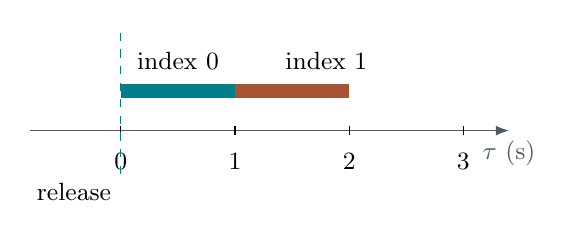
\begin{tikzpicture}[x=1.45cm,y=1cm,font=\small,>={Latex}]
\draw[->,ink] (-0.8,0)--(3.4,0) node[below] {$\tau$ (s)};
\foreach \x in {0,1,2,3}{\draw (\x,0.06)--(\x,-0.06) node[below=3pt]{\x};}
\draw[accent,line width=5pt] (0,0.5)--(1,0.5);
\draw[secondary,line width=5pt] (1,0.5)--(2,0.5);
\node[above] at (0.5,0.65){index 0};
\node[above] at (1.8,0.65){index 1};
\draw[accent,dashed] (0,-0.55)--(0,1.3);
\node[anchor=north east] at (0,-0.55){release};
\end{tikzpicture}
\vspace{0.6cm}
\begin{tabular}{rr}\toprule
Horizon (s) & Bar index\\\midrule
1, 10, 60 & 0, 9, 59\\600, 3600 & 599, 3599\\\bottomrule
\end{tabular}
\end{column}\end{columns}
\source{ADR 0004: returns use the close of bar $\tau-1$; the likelihood uses elapsed time $\tau$, never the bar index.}
\end{frame}

\begin{frame}{Observed returns and the modelled response}
\begin{align*}
R_e(\tau)&=\log P_e(\tau)-\log P_e(0^-),\\[0.4em]
R_e(\tau)&=\underbrace{m_e(\tau)}_{\text{modelled mean}}+
\underbrace{\varepsilon_e(\tau)}_{\text{background movement}}.
\end{align*}
\begin{itemize}
\item $m_e(\tau)$ is the expected return conditional on event $e$'s parameters, not an average of up and down releases.
\item Observe cumulative returns at $\mathcal T=\{1,10,60,600,3600\}$ seconds.
\item $H=3600$ s is the terminal horizon; $M_e:=m_e(H)$ is the signed terminal magnitude.
\item Log returns are dimensionless; $10^4R_e$ expresses them in basis points (bp).
\end{itemize}
\source{The mean is a model component, not an identified causal effect of the release alone.}
\end{frame}

\begin{frame}{The estimand: fraction of the expected terminal move}
\[\phi_e(\tau):=\frac{m_e(\tau)}{m_e(H)}=\frac{m_e(\tau)}{M_e},\qquad M_e\ne0.\]
\begin{columns}[T,onlytextwidth]
\begin{column}{0.47\textwidth}\heading{What it measures}
\begin{itemize}
\item The expected fraction reached by $\tau$, relative to the one-hour destination.
\item Magnitude cancels; a falling response can have the same fraction as a rising one.
\item $\phi_e(H)=1$ by definition, not as an empirical finding.
\end{itemize}\end{column}
\begin{column}{0.47\textwidth}\heading{What it does not measure}
\begin{itemize}
\item The fraction of an observed return, $R_e(\tau)/R_e(H)$.
\item Distance to an independently observed efficient price.
\item Speed identified from a zero response: at $M_e=0$, the data contain no rate information.
\end{itemize}\end{column}\end{columns}
\source{ADR 0002; \texttt{docs/framings/fraction-of-move.md}.}
\end{frame}

\begin{frame}{Why averaging observed ratios fails}
For $E$ events in the fitted sample,
\[\widehat\phi(\tau)=\frac1E\sum_{e=1}^E\frac{R_e(\tau)}{R_e(H)}
\qquad\text{is not the chosen estimand.}\]
\begin{columns}[T,onlytextwidth]
\begin{column}{0.47\textwidth}\heading{Noisy denominator}
\begin{itemize}
\item A one-hour return near zero produces an arbitrarily large ratio.
\item Averaging does not remove this instability; the ratio's expectation need not exist.
\end{itemize}\end{column}
\begin{column}{0.47\textwidth}\heading{Selection is not a repair}
\begin{itemize}
\item Dropping small one-hour returns selects on a post-release outcome.
\item Fit magnitude and rate jointly instead; retain every event meeting the data rules.
\end{itemize}\end{column}\end{columns}
\source{Avoiding division by data removes this estimator's failure. It does not guarantee that every event's rate is identified.}
\end{frame}

\begin{frame}{Response curve: one magnitude and one rate per event}
\begin{columns}[c,onlytextwidth]
\begin{column}{0.52\textwidth}
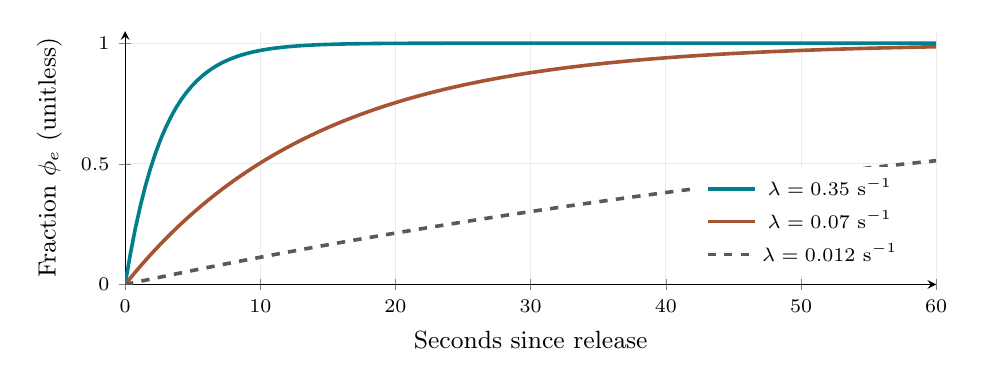
\begin{tikzpicture}
\begin{axis}[width=0.98\textwidth,height=4.8cm,xmin=0,xmax=60,ymin=0,ymax=1.05,
 xlabel={Seconds since release},ylabel={Fraction $\phi_e$ (unitless)},
 legend pos=south east,legend style={fill=white}]
\addplot[accent,domain=0:60,samples=160]{(1-exp(-0.35*x))/(1-exp(-0.35*3600))};
\addlegendentry{$\lambda=0.35\ \mathrm{s}^{-1}$}
\addplot[secondary,domain=0:60,samples=160]{(1-exp(-0.07*x))/(1-exp(-0.07*3600))};
\addlegendentry{$\lambda=0.07\ \mathrm{s}^{-1}$}
\addplot[ink,dashed,domain=0:60,samples=160]{(1-exp(-0.012*x))/(1-exp(-0.012*3600))};
\addlegendentry{$\lambda=0.012\ \mathrm{s}^{-1}$}
\end{axis}\end{tikzpicture}
\end{column}
\begin{column}{0.45\textwidth}
\[m_e(\tau)=M_e\frac{1-e^{-\lambda_e\tau}}{1-e^{-\lambda_e H}}\]
\begin{itemize}
\item $\lambda_e>0$ is the rate, in $\mathrm{s}^{-1}$: larger means faster.
\item Normalisation ensures $m_e(H)=M_e$, not merely an asymptotic limit.
\item One monotone response: the form cannot represent overshoot or reversal.
\end{itemize}\end{column}\end{columns}
\source{Curves illustrate the model at fixed rates; they are not fitted results.}
\end{frame}

\begin{frame}{Half-time: solve for half the terminal response}
\begin{columns}[c,onlytextwidth]
\begin{column}{0.51\textwidth}
\begin{align*}
\phi_e(\tau_{1/2})&=\tfrac12\\[0.4em]
1-e^{-\lambda_e\tau_{1/2}}&=\tfrac12(1-e^{-\lambda_e H})\\[0.4em]
e^{-\lambda_e\tau_{1/2}}&=\tfrac12(1+e^{-\lambda_e H})\\[0.4em]
\tau_{1/2}(\lambda_e)&=\frac1{\lambda_e}\log\frac2{1+e^{-\lambda_e H}}.
\end{align*}\end{column}
\begin{column}{0.43\textwidth}\begin{itemize}
\item Half-time is in seconds and decreases as the rate increases.
\item If $\lambda_e H$ is large, $\tau_{1/2}\approx\log 2/\lambda_e$.
\item As $\lambda_e\to0$, the normalised path becomes linear and half-time tends to $H/2$.
\item Below one second, a half-time is an extrapolation from the curve, not resolved timing.
\end{itemize}\end{column}\end{columns}
\end{frame}

\begin{frame}{Likelihood: the five returns are one observation vector}
\[\mathbf R_e=(R_e(\tau_1),\ldots,R_e(\tau_5))^\top
\sim\mathcal N(\mathbf m_e,\Sigma_e),\qquad
\Sigma_{e,jk}=\varsigma_e^2\min(\tau_j,\tau_k).\]
\begin{itemize}
\item $\mathbf m_e$ contains the response curve at the five horizons.
\item $\varsigma_e$ is event-specific background volatility, in return units per $\sqrt{\mathrm{s}}$.
\item The covariance assumes zero-mean, independent background increments with variance proportional to elapsed time.
\item Different events are conditionally independent given their parameters and the population parameters.
\end{itemize}
\source{These are assumptions of the likelihood. Jumps, changing within-hour volatility and baseline noise can violate them.}
\end{frame}

\begin{frame}{Nested horizons share the same early increments}
\begin{columns}[T,onlytextwidth]
\begin{column}{0.48\textwidth}
For the first three horizons:
\[\Sigma_e=\varsigma_e^2\begin{pmatrix}1&1&1\\1&10&10\\1&10&60\end{pmatrix}.\]
\begin{itemize}
\item Diagonal: variance at each elapsed time.
\item Off-diagonal: variance accumulated during the shared interval.
\end{itemize}\end{column}
\begin{column}{0.46\textwidth}
Write the 60-second noise as
\[\varepsilon_e(60)=\varepsilon_e(10)+\Delta_e(10,60),\]
where the later increment is independent. Then
\[\begin{aligned}
&\operatorname{Cov}\{\varepsilon_e(10),\varepsilon_e(60)\}\\
&\qquad=\operatorname{Var}\{\varepsilon_e(10)\}=10\varsigma_e^2.
\end{aligned}\]
\begin{itemize}\item A diagonal covariance incorrectly treats the shared movement as fresh evidence.\end{itemize}
\end{column}\end{columns}
\source{Equivalent implementation: independent return increments, with variances $\varsigma_e^2(\tau_k-\tau_{k-1})$, $\tau_0=0$.}
\end{frame}

\begin{frame}{Partial pooling: event rates come from one population}
\[\log\lambda_e\sim\mathcal N(\mu,\sigma^2),\qquad
\log\lambda_e=\mu+\sigma z_e,\quad z_e\sim\mathcal N(0,1).\]
\begin{columns}[T,onlytextwidth]
\begin{column}{0.47\textwidth}\heading{Population parameters}
\begin{itemize}
\item $\mu$: centre of log rates; $\exp(\mu)$ is the population median rate.
\item $\sigma$: between-event spread of log rates, not posterior uncertainty about $\mu$.
\item The second expression is the non-centred form used for sampling.
\end{itemize}\end{column}
\begin{column}{0.47\textwidth}\heading{Why pool?}
\begin{itemize}
\item Separate rates allow events to differ.
\item Weak events borrow information from the population rather than being discarded.
\item Strong shrinkage is not evidence that a weak event has a well-measured rate.
\end{itemize}\end{column}\end{columns}
\source{Rate priors: $\mu\sim\mathcal N(-2.7,1.5^2)$ and $\sigma\sim\mathrm{HalfNormal}(1)$, with time in seconds.}
\end{frame}

\begin{frame}{How pooling weights an event's evidence}
\begin{columns}[T,onlytextwidth]
\begin{column}{0.52\textwidth}\heading{Local Gaussian approximation}
Let $\theta_e=\log\lambda_e$, and suppose
\[\widehat\theta_e\mid\theta_e\sim\mathcal N(\theta_e,s_e^2),\qquad
\theta_e\sim\mathcal N(\mu,\sigma^2).\]
With $\mu,\sigma$ fixed, the posterior mean is
\[\mathbb E[\theta_e\mid\widehat\theta_e]
=w_e\widehat\theta_e+(1-w_e)\mu,\]
\[w_e=\frac{\sigma^2}{\sigma^2+s_e^2}.\]
\end{column}
\begin{column}{0.42\textwidth}\begin{itemize}
\item Small event uncertainty $s_e$: more weight on the event estimate.
\item Large $s_e$: more weight on the population centre.
\item Larger population spread $\sigma$: less shrinkage.
\item The actual nonlinear fit estimates event and population parameters jointly.
\end{itemize}\end{column}\end{columns}
\source{The formula explains the weighting mechanism; it is not a replacement likelihood.}
\end{frame}

\begin{frame}{Priors: the specification is not yet ready for estimation}
\begin{columns}[T,onlytextwidth]
\begin{column}{0.47\textwidth}\heading{Preregistered}
\begin{itemize}
\item Log-normal rate hierarchy with the priors on the preceding slides.
\item $\log|M_e|\sim\mathcal N(\mu_M,\sigma_M^2)$, but ``sign free'' is not a complete signed prior.
\item $\log\varsigma_e\sim\mathcal N(\nu,\omega^2)$; volatility varies across events.
\end{itemize}\end{column}
\begin{column}{0.47\textwidth}\heading{Decisions still open}
\begin{itemize}
\item Consistent model units and a continuous signed-magnitude prior (\#31).
\item Volatility priors and the prior-predictive bound, informed by candidate simulations (\#42).
\item Residual and robustness definitions (\#43); concurrent-release treatment (\#32).
\end{itemize}\end{column}\end{columns}
\source{Proposals are not adopted specifications. ADRs and a dated deviation (\#44) must precede implementation and real-data fitting.}
\end{frame}

\begin{frame}{Posterior inference: sample the joint uncertainty}
\[p(\Theta\mid\mathbf R)\propto
\underbrace{p(\Theta)}_{\text{priors and hierarchies}}
\prod_{e=1}^E\underbrace{p(\mathbf R_e\mid\Theta)}_{\text{joint likelihood for event }e}.\]
\begin{itemize}
\item $\Theta$ collects all event and population parameters. One posterior draw gives one value for each.
\item The rate enters nonlinearly; numerical sampling replaces analytic posterior integration.
\item NumPyro's No-U-Turn Sampler (NUTS) uses gradients to explore the posterior and chooses a trajectory length for each draw.
\item Four chains start separately: 1000 warmup iterations, then 2000 retained draws each; acceptance target 0.8.
\end{itemize}
\source{Warmup adapts the sampler and is discarded. The retained draws are correlated; diagnostics assess their numerical reliability.}
\end{frame}

\begin{frame}{Posterior summaries: transform every draw, then take quantiles}
For retained draw $s$, compute
\[\lambda_{\mathrm{pop}}^{(s)}=e^{\mu^{(s)}},\qquad
t_{\mathrm{pop}}^{(s)}=\frac1{\lambda_{\mathrm{pop}}^{(s)}}
\log\frac2{1+e^{-\lambda_{\mathrm{pop}}^{(s)}H}}.\]
\begin{itemize}
\item Report the median and the 2.5th and 97.5th percentiles of $t_{\mathrm{pop}}^{(s)}$.
\item This is the posterior of the population median half-time, not the mean of estimated event half-times.
\item Similarly, report $\phi(\tau;e^{\mu^{(s)}})$ at each horizon, plus $\mu$ and $\sigma$, with 95\% credible intervals.
\item A credible interval describes parameter uncertainty under the model; it is not the spread of event half-times.
\end{itemize}
\source{The population curve uses the median rate. It is not $\mathbb E_{\lambda}[\phi(\tau;\lambda)]$, the mean curve over events.}
\end{frame}

{\setbeamertemplate{footline}{}
\begin{frame}[plain]
\vspace{1cm}{\color{accent}\rule{1.4cm}{2pt}}\par\vspace{0.6cm}
{\huge Part 2: Validation and interpretation}\par\vspace{0.6cm}
Pre-data gates, diagnostics, robustness and permitted claims
\end{frame}}

\begin{frame}{Before real-data fitting: plausibility and recovery}
\begin{columns}[T,onlytextwidth]
\begin{column}{0.47\textwidth}\heading{Prior predictive}
\begin{itemize}
\item Draw population parameters, then event parameters, then returns.
\item Preregistered criterion: at least 95\% of $|R(H)|$ below 500 bp.
\item The bound's justification needs correction: the exploratory grid was not a one-hour sample.
\item Candidate priors and bounds are assessed before a choice is logged.
\end{itemize}\end{column}
\begin{column}{0.47\textwidth}\heading{Recovery}
\begin{itemize}
\item Simulate 100 datasets of 212 events and fit each with the declared settings.
\item Count intervals containing the generating population half-time.
\item Pass band: 90 to 99 of the 100 intervals contain the truth.
\item Report failed fits and divergences too; coverage alone cannot diagnose their cause.
\end{itemize}\end{column}\end{columns}
\source{A failed gate blocks real-data fitting. Repair requires a recorded decision and deviation, then both checks are rerun.}
\end{frame}

\begin{frame}{Fit diagnostics: did sampling characterise the posterior?}
\small\renewcommand{\arraystretch}{1.25}
\begin{tabular}{@{}L{0.23\textwidth}L{0.47\textwidth}L{0.24\textwidth}@{}}\toprule
Diagnostic & What it checks & Preregistered criterion\\\midrule
Rank-normalised split $\widehat R$ & Agreement across chains and their halves & $\widehat R<1.01$\\
Bulk and tail ESS & Effective information in correlated draws, in the centre and tails & Both $>400$\\
Divergences & Numerical failures along sampling trajectories; possible biased exploration & Zero\\\bottomrule
\end{tabular}
\vspace{0.4cm}\begin{itemize}
\item Criteria apply to every parameter as preregistered; proposed scope and tolerance changes remain decisions in \#31.
\item A rejected fit is reported as a study failure, not silently retuned. Passing is necessary, not proof of model validity.
\end{itemize}
\end{frame}

\begin{frame}{Residual shape: can one rate describe the response?}
\begin{columns}[c,onlytextwidth]
\begin{column}{0.51\textwidth}
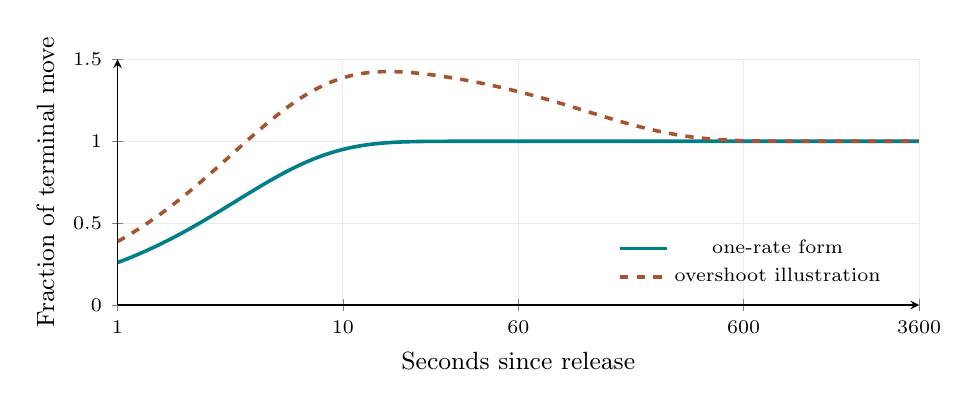
\begin{tikzpicture}
\begin{axis}[width=0.97\textwidth,height=4.7cm,xmode=log,xmin=1,xmax=3600,ymin=0,ymax=1.5,
 xtick={1,10,60,600,3600},xticklabels={1,10,60,600,3600},
 xlabel={Seconds since release},ylabel={Fraction of terminal move},legend pos=south east]
\addplot[accent,domain=1:3600,samples=240]{(1-exp(-0.3*x))/(1-exp(-0.3*3600))};
\addlegendentry{one-rate form}
\addplot[secondary,dashed,domain=1:3600,samples=240]{(1-exp(-0.3*x))*(1+0.5*exp(-x/120))/((1-exp(-0.3*3600))*(1+0.5*exp(-3600/120)))};
\addlegendentry{overshoot illustration}
\end{axis}\end{tikzpicture}
\end{column}
\begin{column}{0.45\textwidth}\begin{itemize}
\item Raw residual: $R_e(\tau_k)-m_e(\tau_k)$ for each event and draw.
\item Scaling, direction alignment and pooling determine which patterns remain visible.
\item ADR 0006 must fix that diagnostic and a numerical overshoot rule before it is applied.
\item Systematic overshoot invalidates a single-rate interpretation; the finding is about shape.
\end{itemize}\end{column}\end{columns}
\source{The dashed curve illustrates a limitation, not the pending two-component specification or an estimated residual pattern.}
\end{frame}

\begin{frame}{Robustness: horizon, functional form and baseline}
\small\renewcommand{\arraystretch}{1.25}
\begin{tabular}{@{}L{0.22\textwidth}L{0.36\textwidth}L{0.36\textwidth}@{}}\toprule
Check & Change & Question\\\midrule
1. Terminal horizon & $H=30$ min and $H=4$ h & Does the chosen destination drive the half-time?\\
2. Functional form & Add an overshoot-capable response & Does it improve held-out predictive density?\\
3. Baseline & Mean price over the preceding 10 s & How sensitive is the curve to the last pre-release trade?\\\bottomrule
\end{tabular}
\vspace{0.4cm}\begin{itemize}
\item The four-hour arm admits later scheduled news; it cannot establish isolated-release timing.
\item Horizon grids, the alternative model and predictive comparison are fixed in ADR 0006, not chosen after fitting.
\end{itemize}
\end{frame}

\begin{frame}{Robustness: population structure and prior sensitivity}
\small\renewcommand{\arraystretch}{1.2}
\begin{tabular}{@{}L{0.22\textwidth}L{0.36\textwidth}L{0.36\textwidth}@{}}\toprule
Check & Change & Interpretation\\\midrule
4. Release type & Allow different log-rate centres & CPI versus Employment Situation; secondary\\
5. Time & Linear year trend in log rate & Change across sample years; secondary\\
6. Rate prior & $\mu\sim\mathcal N(0,3^2)$ & Sensitivity to reuse of exploratory dates\\
7. FOMC & Separate statement sample & Contaminated by the press conference\\\bottomrule
\end{tabular}
\vspace{0.2cm}\begin{itemize}
\item Wide subgroup or trend intervals are reported as wide, not read as evidence of no difference.
\item All seven checks remain planned. A concurrent-release refit requires a deviation (\#32, \#44).
\end{itemize}
\end{frame}

\begin{frame}{Outcome rules: failures precede the half-time claim}
\begin{enumerate}
\item \textbf{Fit rejected:} the posterior is not characterised. Report the diagnostic failure; no rate claim.
\item \textbf{Overshoot rule fires:} one rate does not describe the path. Report the shape failure; no rate claim.
\item \textbf{Otherwise:} classify the 95\% interval $[L,U]$ for the population half-time.
\end{enumerate}
\vspace{0.5cm}\begin{columns}[T,onlytextwidth]
\begin{column}{0.30\textwidth}\centering\heading{Supported}
$U<60$ s\par\vspace{0.3em}Interval entirely below the threshold.
\end{column}
\begin{column}{0.30\textwidth}\centering\heading{Inconclusive}
$L\le60\le U$\par\vspace{0.3em}Interval includes the threshold.
\end{column}
\begin{column}{0.30\textwidth}\centering\heading{Falsified}
$L>60$ s\par\vspace{0.3em}Interval entirely above the threshold.
\end{column}\end{columns}
\source{Publish null and inconclusive outcomes with the same prominence. Robustness arms qualify the primary verdict, not replace it.}
\end{frame}

\begin{frame}{Interpretation limits}
\begin{itemize}
\item \textbf{Attribution:} other news can enter the window. A fitted response does not identify the effect of CPI or employment news alone.
\item \textbf{Resolution:} one-second bars and an unverified exchange-clock offset limit the shortest measurable times.
\item \textbf{Shape:} the half-time is conditional on the exponential form and the chosen terminal horizon.
\item \textbf{Weak events:} a small magnitude leaves little rate information; a concentrated hierarchical posterior can be driven by pooling or priors.
\item \textbf{Scope:} one asset, one venue and primary releases at 08:30 ET. No inference about all markets follows.
\end{itemize}
\source{No empirical precision or gate outcome is claimed here. Full objections and planned checks: \texttt{docs/limitations.md}.}
\end{frame}

\begin{frame}{What a completed measurement must report}
\begin{itemize}
\item Population half-time and incorporation curve with 95\% intervals, only where the outcome rules permit interpretation.
\item Exclusion counts and reasons; pre-data gate results; fit diagnostics; residual verdict.
\item Every planned robustness result, including rejected fits and analyses not run.
\item Deviations from the original plan, with their reasons and the claims they change.
\end{itemize}
\vspace{0.5cm}\heading{Current stopping point}
The estimand is fixed. Specification decisions and validation gates remain open. No primary half-time has been estimated.
\source{Audit trail: \texttt{PREREGISTRATION.md}, ADRs 0001 to 0004, and issues \#31, \#32, \#42 to \#45.}
\end{frame}

\appendix
\begin{frame}{Backup: preregistered exclusions}
An event is excluded only for a declared data failure:
\begin{enumerate}
\item The daily archive is missing or fails checksum verification.
\item Fewer than 95\% of seconds in $[-300,+3600]$ carry a trade.
\item No trade occurs in the 60 seconds before release.
\end{enumerate}
\vspace{0.5cm}\begin{itemize}
\item No exclusion for a small terminal move, unexpected sign, implausible rate or poor fit.
\item Missing grid-second handling is still to be fixed in ADR 0006.
\item Concurrent-release treatment is a separate pending decision; any exclusion requires a logged sample change.
\end{itemize}
\end{frame}

\begin{frame}{Backup: the original prior table and its unresolved parts}
\small\renewcommand{\arraystretch}{1.1}
\begin{tabular}{@{}L{0.21\textwidth}L{0.45\textwidth}L{0.28\textwidth}@{}}\toprule
Parameter & Preregistered distribution & Status\\\midrule
$\mu$ & $\mathcal N(-2.7,1.5^2)$ & Rate prior retained\\
$\sigma$ & $\mathrm{HalfNormal}(1)$ & Rate spread retained\\
$\mu_M$ & $\mathcal N(\log30,1^2)$ & Intended magnitude: bp\\
$\sigma_M$ & $\mathrm{HalfNormal}(1)$ & Incomplete sign prior\\
$\nu$ & $\mathcal N(0,2^2)$ & Volatility location\\
$\omega$ & $\mathrm{HalfNormal}(1)$ & Volatility spread\\\bottomrule
\end{tabular}
\vspace{0.35cm}\begin{itemize}
\item $\log|M_e|\sim\mathcal N(\mu_M,\sigma_M^2)$ and $\log\varsigma_e\sim\mathcal N(\nu,\omega^2)$.
\item The table's numerical scales and dimensionless returns are not consistent without an explicit unit conversion. ADR 0005 must resolve this and supply a signed prior.
\end{itemize}
\source{Original plan reproduced for audit, not presented as an executable model. Candidate changes are not adopted by this deck.}
\end{frame}

\begin{frame}{Sources and further detail}
\begin{itemize}
\item \textbf{Analysis contract:} \texttt{PREREGISTRATION.md}, including its dated sample-count deviation.
\item \textbf{Model and notation:} \texttt{docs/framings/}; \textbf{limits:} \texttt{docs/limitations.md}.
\item \textbf{Release and alignment decisions:} \texttt{docs/adr/0001} to \texttt{0004}.
\item \textbf{NUTS:} Hoffman and Gelman (2014), \emph{The No-U-Turn Sampler}, JMLR 15, 1593 to 1623.
\item \textbf{Diagnostics:} Vehtari et al. (2021), \emph{Rank-Normalization, Folding, and Localization}, Bayesian Analysis 16(2), 667 to 718.
\end{itemize}
\end{frame}
\end{document}